
% ------------------------------------------------------------
% ------------------------------------------------------------

%%%%%%%%%%%%%%%%%%%%%%%%%%%%%%%%%%%%%
\section{Simulation Plots}
\subsection{Preliminaries}
%_______________________

\begin{frame}[fragile]
\frametitle{Simulations}
\framesubtitle{Preliminaries: The function \ttfamily outer() \normalfont}

    \begin{columns}[Tc]
      \column{0.42\textwidth}
\begin{lstlisting}
x=5:6; y=1:3
outer(x,y)
\end{lstlisting}

\begin{beamerboxesrounded}[shadow=true]{}
\ttfamily
\begin{verbatim}
     [,1] [,2] [,3] 
[1,]    5   10   15 
[2,]    6   12   18 
\end{verbatim}
\end{beamerboxesrounded}
\normalfont

	     \column{0.58\textwidth}
\begin{lstlisting}
fcn<-function(x,y){z=x+y}
outer(x,y,fcn)
\end{lstlisting}

\begin{beamerboxesrounded}[shadow=true]{}
\ttfamily
\begin{verbatim}
     [,1] [,2] [,3] 
[1,]    6    7    8 
[2,]    7    8    9 
\end{verbatim}
\end{beamerboxesrounded}
\normalfont
	\end{columns}
\end{frame}

%%%%%%%%%%%%%%%%%%%
\subsection{Performing the Simulation and Visualizing the Results}
%________________________________
\begin{frame}[fragile, allowframebreaks]
\frametitle{Simulations}
\framesubtitle{Visualize with \ttfamily persp() \normalfont}

Suppose we want to know what the function $y\times sin(x)$ looks like:

\begin{lstlisting}
# Sample from the random uniform:
x <- sort(runif(100, min=0, max=10))
y <- x+runif(1)
f <- function(x,y) { r <- y*sin(x)}
z <- outer(x,y,f)
persp(x, y, z, col = "lightblue", shade = 0.1, ticktype = "detailed", expand=0.7)
\end{lstlisting}
% set.seed(04262010)

\newpage
   \begin{figure}[ht]
       \begin{center}
		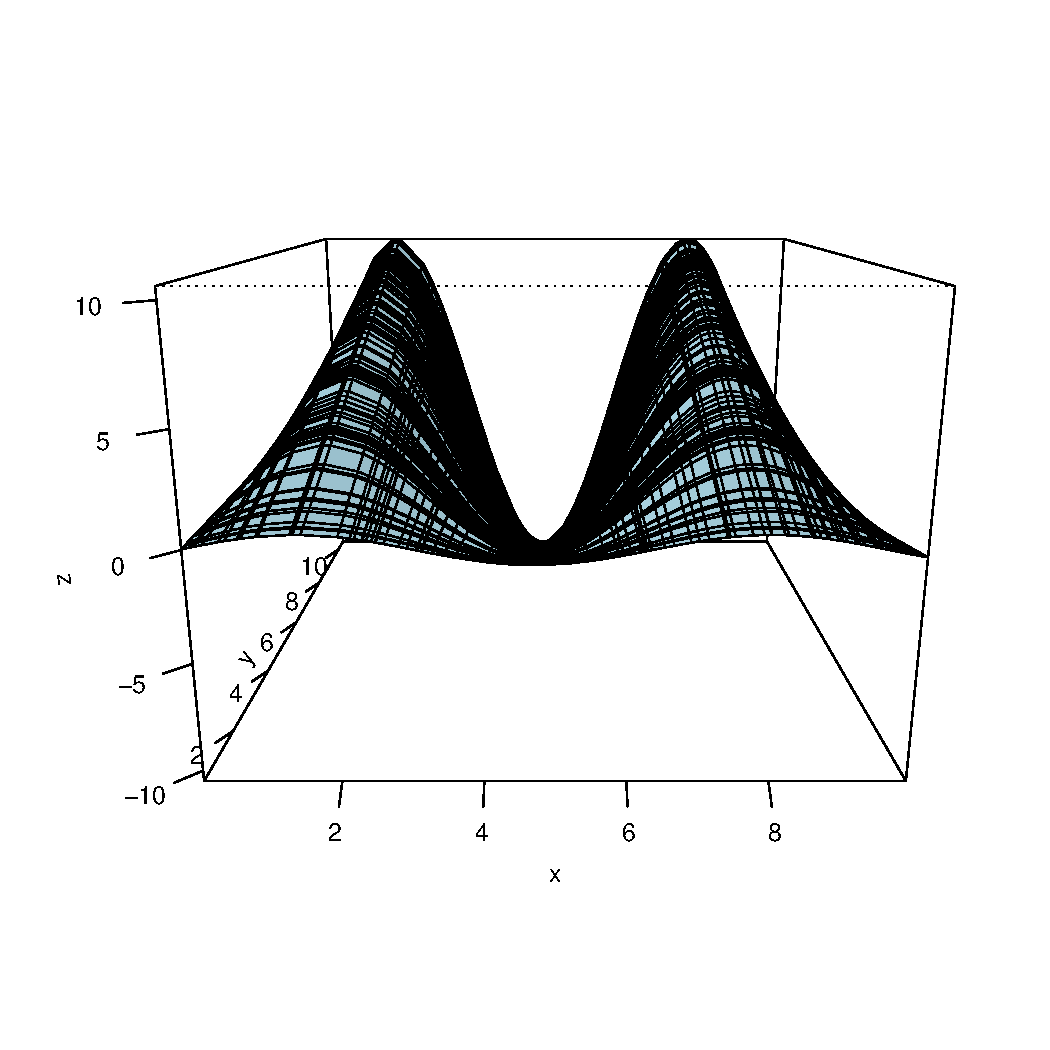
\includegraphics[width = 3.5in]{images/simulation.png}
	\end{center}
   \end{figure}
\end{frame}

%_________
\begin{frame}[fragile, allowframebreaks]
\frametitle{Simulations}
\framesubtitle{Visualize with \ttfamily image() \normalfont}

To visually see its maximum and minimum values, look at the contours of the function:

\begin{lstlisting}
# Format the data appropriate for the image() function:
x.seq<-seq(from=range(x)[1], to=range(x)[2], length=100)
y.seq<-seq(from=range(y)[1], to=range(y)[2], length=100)
n1<-length(x.seq)
n2<-length(y.seq)
mat1<-matrix(z, nrow=n1, ncol=n2, byrow=FALSE)
image(x.seq, y.seq, mat1)
contour(x.seq, y.seq, mat1, add=TRUE)
\end{lstlisting}

\newpage
   \begin{figure}[ht]
       \begin{center}
		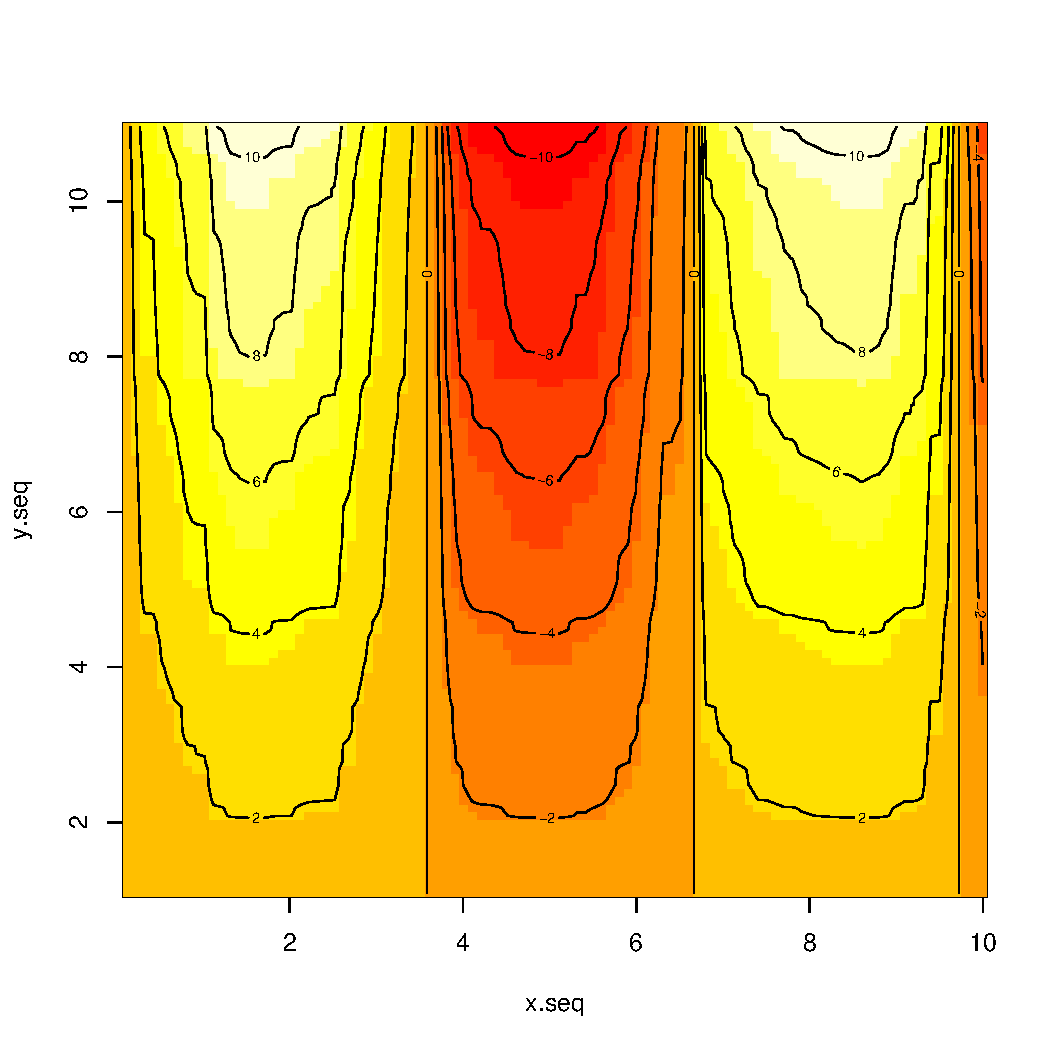
\includegraphics[width = 2.5in]{images/contourSim.pdf}
	\end{center}
   \end{figure}
\end{frame}

%g <- expand.grid(x = 1:10, y = 5:15)
%g$z<-g$x^2
%wireframe(g$z~g$x*g$y, scales = list(arrows = FALSE), drape = TRUE, colorkey = TRUE)

\begin{frame}[fragile, allowframebreaks]
\frametitle{Simulations}
\framesubtitle{Visualize with \ttfamily plot3d() \normalfont}

Suppose we want to know what the function $y\times sin(x)$ looks like with a dynamic plot:

\begin{lstlisting}
# Sample from the random uniform:
x1 <- sort(runif(10000, min=0, max=10))
y1 <- x1+runif(1000, min=0,  max=20)
z1<-y1*sin(x1)
librray(rgl)
plot3d(x1, y1, z1)

\end{lstlisting}

\newpage
   \begin{figure}[ht]
       \begin{center}
		\includegraphics[width = 2in]{images/plot3dSin1.png}
		\includegraphics[width = 2in]{images/plot3dSin2.png}
	\end{center}
   \end{figure}
\end{frame}


% ------------------------------------------------------------
% ------------------------------------------------------------
\subsection{Exercise V}
\begin{frame}
	\frametitle{Exercise V}
	Visualize the following function:
	\begin{equation}
		z \hspace{0.01in} =\hspace{0.01in} \frac{sin(\frac{3}{2}x)}{y}
	\end{equation}	
\end{frame}

%# Sample from the random uniform:
%x <- sort(runif(100, min=0, max=10))
%y <- x+runif(1)
%f <- function(x,y) { r <- sin(1.5*x)/y}
%z <- outer(x,y,f)
%persp(x, y, z, col = terrain.colors(length(z)/4), shade = 0.1, ticktype = "detailed", expand=0.7)